\documentclass{report}
% PACKAGES
\usepackage[utf 8]{inputenc }
\usepackage {mathtools} % math and figures
\usepackage {float} % places figure at point with [H]
\usepackage {filecontents}
\usepackage [numbered,framed]{matlab-prettifier}
% these packages include more math symbols you might use
\usepackage { amsmath , amsfonts , amsthm , amssymb }
% PROJECT Specific Information to Fill Out
\newcommand{\LectureTitle}{Forecasting Financial Market}
\newcommand{\LectureDate }{\today }
\newcommand{\LectureClassName }{ECON 623}
\newcommand{\LatexerName }{Zixin Huang}
\author {Zixin Huang }

% CONFIGURATIONS to make the report look better
\usepackage { setspace }
\usepackage { Tabbing }
\usepackage { fancyhdr }
\usepackage { lastpage }
\usepackage { extramarks }
\usepackage { afterpage }
\usepackage { abstract }
% In case you need to adjust margins :
\topmargin = -0.45 in
\evensidemargin =0 in
\oddsidemargin =0 in
\textwidth =6.5 in
\textheight =9.0 in
\headsep =0.25 in
% Setup the header and footer
\pagestyle{fancy}
\lhead{\LatexerName }
\chead{\LectureClassName : \LectureTitle }
\rhead{\LectureDate }
%\lfoot{\astxmark }
%\cfoot{}
%\rfoot{ Page \ \ thepage \ of \ \ pageref { LastPage }}
\renewcommand\headrulewidth {0.4 pt }
\renewcommand\footrulewidth {0.4 pt }




\usepackage{indentfirst}
\title {\LectureTitle : Homework 1}

\begin{document}
	
\maketitle

\section*{Question 1}

\subsection*{a}
I used the time series data of the USD/Euro Exchange rate and the S\&P 500 from 2015-01-21 to 2019-01-21.

\begin{figure}[H]
	\centering
	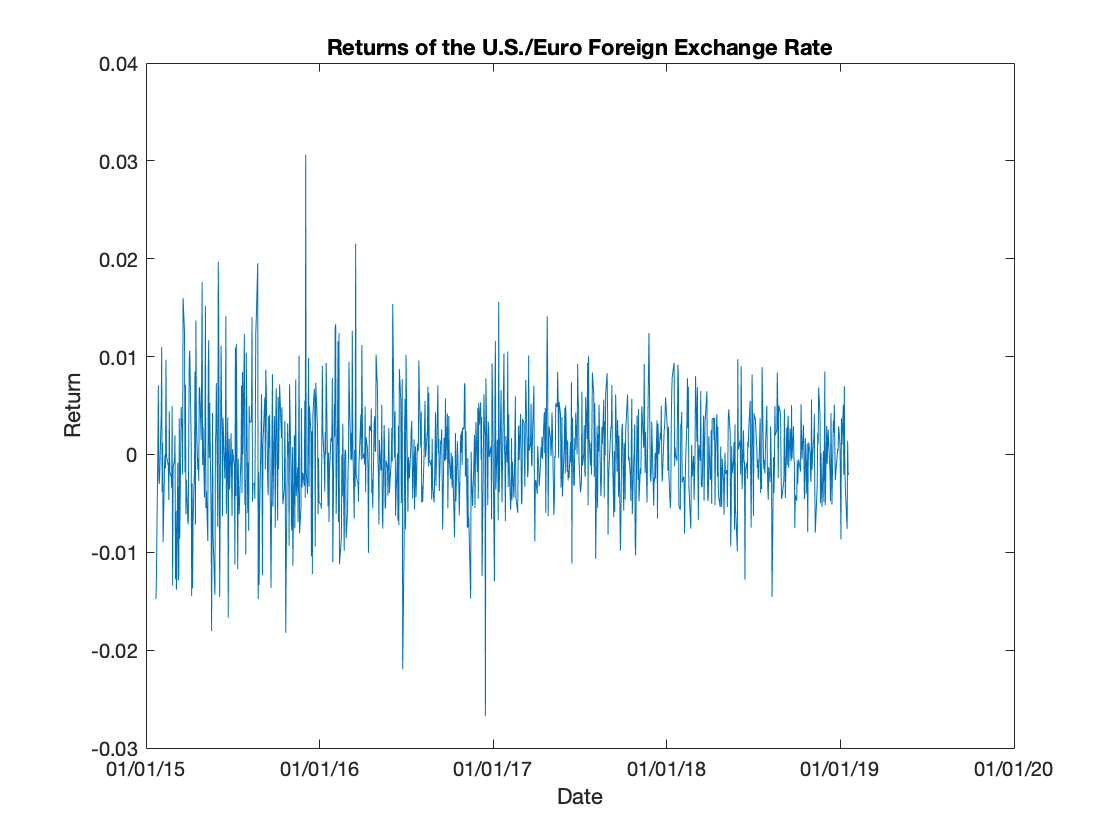
\includegraphics[width = 11cm]{1a1}
	\caption{Continuously Compounded Returns of the USD/Euro Exchange Rate} 
\end{figure}

\begin{figure}[H]
	\centering
	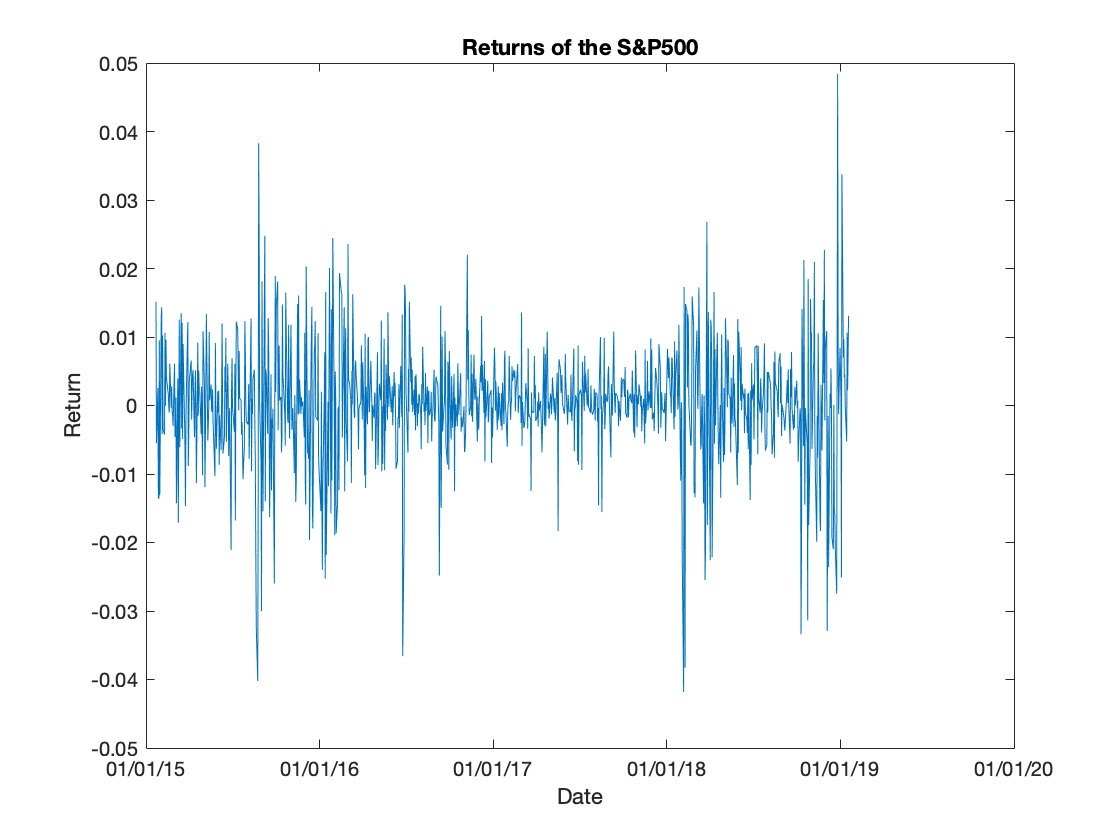
\includegraphics[width = 11cm]{1a2}
	\caption{Continuously Compounded Returns of the S\&P500} 
\end{figure}

\subsection*{b}

 \begin{table}[H]
	\begin{center}
		\caption{Summary Statistics}
		\label{tab:table1}
		\vspace{2mm}
		\begin{tabular}{c|c|c|c|c|c|c|c|} 
			
		%	\specialrule{.1em}{.1em}{0em}
			
			\textbf{Asset} & \textbf{mean}&  \textbf{median}& \textbf{maximum}&\textbf{minimum}&\textbf{STD}&\textbf{skewness}&\textbf{kurtosis}\\
			\hline
			
			DEXUSEU &  $-1.9370\times 10^{-5}$& $-2.5341\times 10^{-4}$&$0.0306$&$-0.0267$ &$0.0056$&$0.1047$ &$5.0468$   \\
			
			SP500 & $2.7163\times 10^{-4}$&$3.4225\times 10^{-4}$ &$0.0484$&$-0.0418$&$0.0087$&$-0.4698$&$7.0125$   \\
			
		%	\specialrule{.1em}{.1em}{0em}
		\end{tabular}
	\end{center}
\end{table}


 \begin{table}[H]
	\begin{center}
		\caption{Jarque-Bera Test}
		\label{tab:table2}
		\vspace{2mm}
		\begin{tabular}{c|c|c|c|} 
			
			%	\specialrule{.1em}{.1em}{0em}
			
			\textbf{Asset} & \textbf{JB test statistic}&  \textbf{JB p-value}& \textbf{JB test result($H$)}\\
			\hline
			
			DEXUSEU &  $176.2116$& $0.001$&$1$   \\
			
			SP500 & $711.8687$&$0.001$ &$1$ \\
			
			%	\specialrule{.1em}{.1em}{0em}
		\end{tabular}
	\end{center}
\end{table}



\lstinputlisting[style = Matlab-editor]{functions/sum_stats.m}

\section*{Exercise 2}

\subsection*{Question a}

 \begin{table}[H]
	\begin{center}
		\caption{Coefficients of the OLS model}
		\label{tab:table3}
		\vspace{2mm}
		\begin{tabular}{c|c|c|c|} 
			
			%	\specialrule{.1em}{.1em}{0em}
			
			\textbf{Parameters} & \textbf{Estimated Value}&  \textbf{SE}& \textbf{t-statistics}\\
			\hline
			
			$\beta_0$ &  $-6.8978\times 10^{-6}$& $0.00017771$&$-0.038815$    \\
			$\beta_1$ &  $-0.031506$& $0.020556$&$-1.5327$    \\
			%	\specialrule{.1em}{.1em}{0em}
		\end{tabular}
	\end{center}
\end{table}
R-squared: $0.00236$.  Adjusted R-Squared: $0.00136$.



\subsection*{Question b}

 \begin{table}[H]
	\begin{center}
		\caption{T Test at $5\%$ Significance Level}
		\label{tab:table4}
		\vspace{2mm}
		\begin{tabular}{c|c|c|c|} 
			
			%	\specialrule{.1em}{.1em}{0em}
			
			\textbf{hypothesis} & \textbf{t-statistic}&  \textbf{critical value}& \textbf{result}\\
			\hline
			$H_0:\beta_1=1$ &  $-50.1791$& $1.96$& Reject $H_0$    \\
			%	\specialrule{.1em}{.1em}{0em}
		\end{tabular}
	\end{center}
\end{table}
We are $95\%$ confident to reject the hypothesis that return of the USD/Euro exchange rate move along with the return of the S\&P 500 a day before.


\subsection*{Question c}

 \begin{table}[H]
	\begin{center}
		\caption{Coefficients of the OLS model}
		\label{tab:table5}
		\vspace{2mm}
		\begin{tabular}{c|c|c|c|} 
			
			%	\specialrule{.1em}{.1em}{0em}
			
			\textbf{Parameters} & \textbf{Estimated Value}&  \textbf{SE}& \textbf{t-statistics}\\
			\hline
			
			$\beta_0$ &  $-8.7705\times 10^{-6}$& $0.00017789$&$-0.049302$    \\
			$\beta_1$ &  $-0.027624$& $0.020593$&$-1.3414$    \\
			$\beta_2$ &  $0.0077265$& $0.020581$&$0.37542$    \\
			$\beta_3$ &  $0.030052$& $0.020566$&$1.4612$    \\
			%	\specialrule{.1em}{.1em}{0em}
		\end{tabular}
	\end{center}
\end{table}
R-squared: $0.00429$,  Adjusted R-Squared: $0.00127$

\subsection*{Question d}


\begin{table}[H]
	\begin{center}
		\caption{$\chi^2$ Test at $5\%$ Significance Level}
		\label{tab:table6}
		\vspace{2mm}
		\begin{tabular}{c|c|c|c|} 
			
			%	\specialrule{.1em}{.1em}{0em}
			
			\textbf{hypothesis} & \textbf{$\chi^2$-statistic}&  \textbf{critical value}& \textbf{result}\\
			\hline
			$H_0:\beta_1=\beta_2=\beta_3=0$ &$4.2588$ & $7.8147$& Do not reject $H_0$   \\
			%	\specialrule{.1em}{.1em}{0em}
		\end{tabular}
	\end{center}
\end{table}

We are of $95\%$ confidence to say that we do not reject the null hypothesis that $\beta_1=\beta_2=\beta_3=0$. In other words, we do not reject the hypothesis that return of the USD/Euro exchange rate does not affect by return of the SP500 with neither $1$, $2$, or $3$ lags.

\subsection*{Question e}

\begin{table}[H]
	\begin{center}
		\caption{$\chi^2$ Test at $5\%$ Significance Level}
		\label{tab:table7}
		\vspace{2mm}
		\begin{tabular}{c|c|c|c|} 
			
			%	\specialrule{.1em}{.1em}{0em}
			
			\textbf{hypothesis} & \textbf{$\chi^2$-statistic}&  \textbf{critical value}& \textbf{result}\\
			\hline
			$H_0:\beta_1=\beta_2=\beta_3$ &$4.1805$ &$5.9915$ &Do not reject $H_0$  \\
			%	\specialrule{.1em}{.1em}{0em}
		\end{tabular}
	\end{center}
\end{table}

We are of $95\%$ confidence to say that we do not reject the null hypothesis that $\beta_1=\beta_2=\beta_3$. In other words, we do not reject the hypothesis that the dependence of return of USD/Euro exchange rate on return of SP500 with $1$, $2$, and $3$ lags are the same.


\section*{Question 3}
\subsection*{a}
The theoretical unconditional mean of the AR(1) process can be compute as:

$\mu = E(Y_t)=E(\Phi_0+\Phi_1 Y_{t-1}+\epsilon_t)=\Phi_0+\Phi_1 E(Y_{t-1})=\Phi_0+\Phi_1 \mu$

So $\mu=\frac{\Phi_0}{1-\Phi_1}$.

The MATLAB function I used to generate AR(1) process:

\lstinputlisting[style = Matlab-editor]{functions/AR1.m}

\subsection*{b}

\begin{figure}[H]
	\centering
	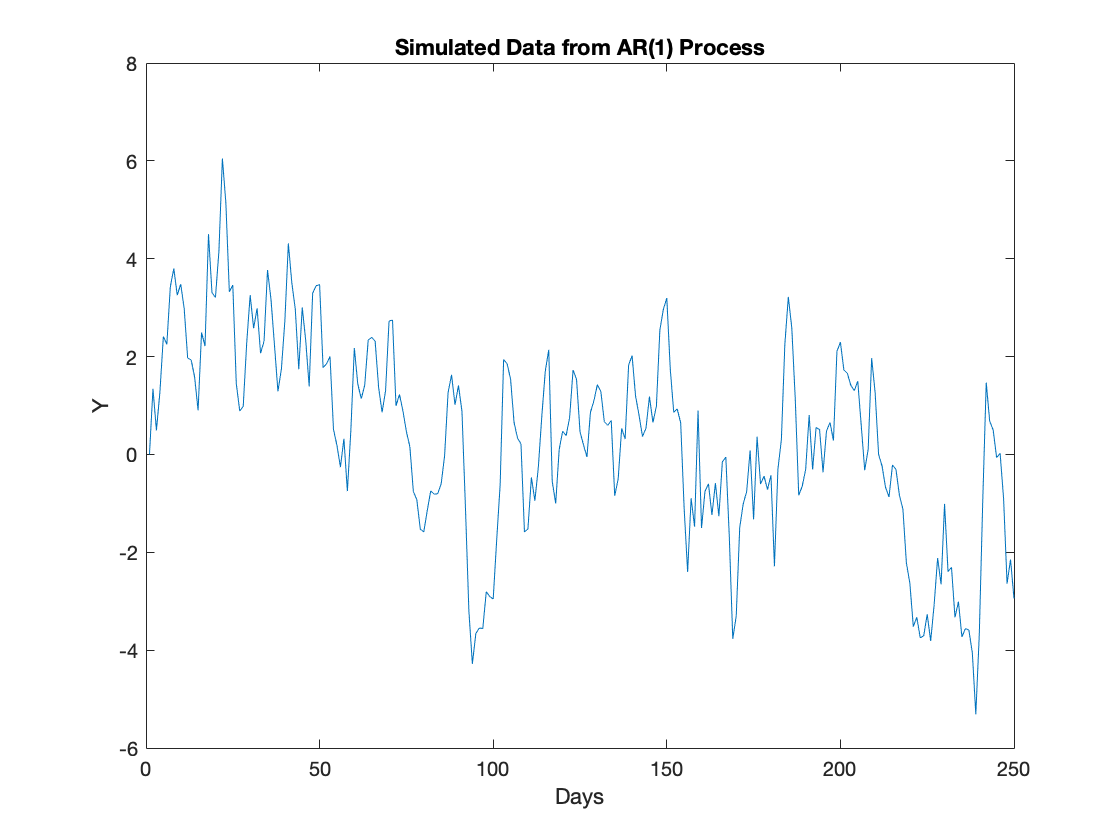
\includegraphics[width = 11cm]{3b}
	\caption{Simulated AR(1) Process with Normally Distributed Innovations} 
\end{figure}

\subsection*{c}

\begin{figure}[H]
	\centering
	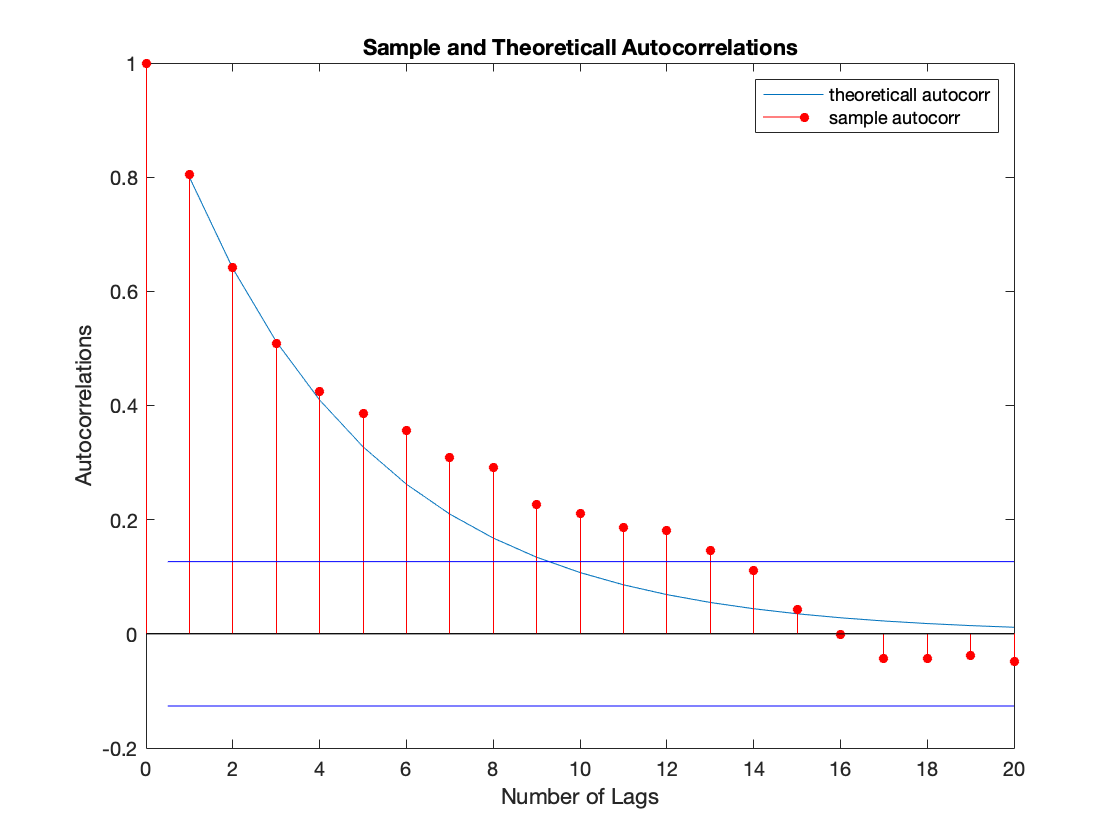
\includegraphics[width = 11cm]{3c}
	\caption{Sample Autocorrelations and Theoretical Autocorrelations of the Simulated Data} 
\end{figure}


Theoretically:

 $\gamma_0=Var(Y_t)=Var(\Phi_0+\Phi_1 Y_{t-1}+\epsilon_t)=\Phi_1^2 Var(Y_{t-1})+Var(\epsilon_t)=\Phi_1^2 \gamma_0+\sigma_\epsilon^2$

So $\gamma_0=\frac{\sigma_\epsilon^2}{1-\Phi_1^2}$

$\gamma_j=\frac{\sigma_\epsilon^2}{1-\Phi_1^2} \Phi_1^j=\gamma_0 \Phi_1^j$

That is $\rho_j=\frac{\gamma_j}{\gamma_0}=\Phi_1^j$.

To compute sample autocorrelations:

$\rho_j=\frac{ \frac{1}{T-j} \sum_{t=j+1}^{T} (y_t-\bar{y})(y_{t-j}-\bar{y})}{ \frac{1}{T} \sum_{t=1}^{T} (y_t-\bar{y})^2  }$.

\lstinputlisting[style = Matlab-editor]{Q3.m}

\section*{Question 4}

\subsection*{a}

\lstinputlisting[style = Matlab-editor]{functions/AR1_uni.m}

\subsection*{b}

\begin{figure}[H]
	\centering
	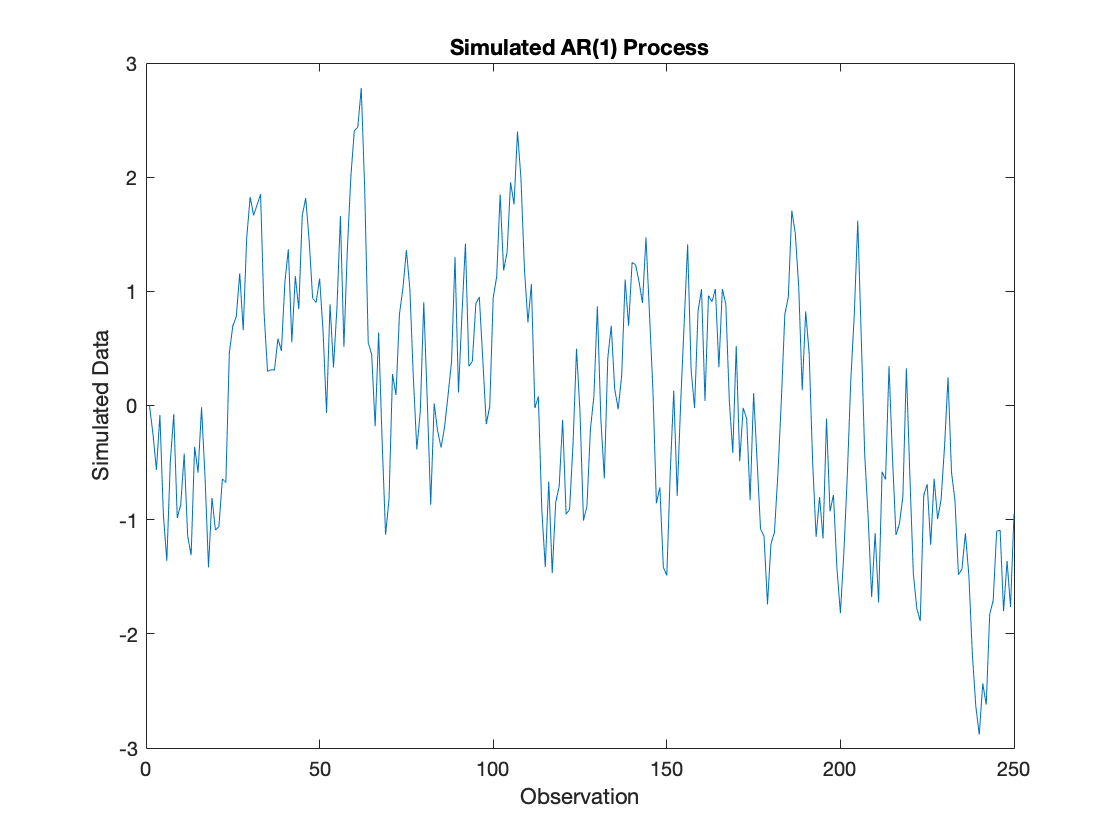
\includegraphics[width = 11cm]{4b}
	\caption{Simulated AR(1) Process with Uniformly Distributed innovations} 
\end{figure}

\subsection*{c}

$E(X_t) = \mu = \frac{\phi_0}{1-\phi_1}+\frac{U+L}{2(1-\phi_1)}$

\subsection*{d}
 \begin{table}[H]
	\begin{center}
		\caption{Sample and Theoretical mean of the AR(1) Process}
		\label{tab:table8}
		\vspace{2mm}
		\begin{tabular}{c|c|c} 
			
			%	\specialrule{.1em}{.1em}{0em}
			
			\textbf{Parameters} & \textbf{Sample Mean}&  \textbf{$E(X_t)$}\\
			\hline
			
			$(0,0.8,-1,1)$ &  $-7.8386\times 10^{-4}$& $0$    \\
			$(0,0.8,-2,1)$ &  $-2.4967$& $-2.5$  \\
			$(1,0.8,-5,2)$ &  $-2.5076$& $-2.5$  \\
			%	\specialrule{.1em}{.1em}{0em}
		\end{tabular}
	\end{center}
\end{table}
From the table we can see that when  $T=1000,000$ the sample mean is very close to the unconditional expectation for each of these three scenarios.


\end{document}